\chapter{Anhang}
\label{chap:Anhang}
\section{Ergebnisse der statischen und dynamischen Messung ohne Reglerveränderung}\label{sec:MessergebnisseOhneRegleranderung}

\begin{longtable}[]{llllllll}
\caption{Ergebnisse der statischen Messung}
\tabularnewline
\toprule
Last  & PF    & $S_{\mathrm{gen}}$ (kVA) & $P_{\mathrm{gen}}$ (kW) & $I_{\mathrm{gen}}$ (A) & $U_{\mathrm{pol.}}$ (V) & $U_{\mathrm{gen}}$ (V) & $U_{\mathrm{err.}}$ (V) \\ 
\midrule
\endhead
\unit[0]{\%}   & 1,0   & 0          & 0         & 0        &           & 115,3    & 15,2      \\
\unit[25]{\%}  & 1,0   & 17,8       & 17,8      & 51,4     &           & 115,2    & 15,5      \\
\unit[50]{\%}  & 1,0   & 36,2       & 36,2      & 104,7    &           & 115,1    & 16,3      \\
\unit[75]{\%}  & 1,0   & 54,1       & 54,1      & 156,8    &           & 115,1    & 17,4      \\
\unit[100]{\%} & 1,0   & 71,6       & 71,6      & 207,6    &           & 115,0    & 18,4      \\
\unit[125]{\%} & 1,0   & 90,3       & 90,3      & 262,0    &           & 114,9    & 20,0      \\
\unit[150]{\%} & 1,0   & 107,3      & 107,3     & 311,3    &           & 114,8    & 21,4      \\ \midrule
\unit[0]{\%}   & 0     & 0          & 0         & 0        & 50,4      & 115,5    & 12,5      \\
\unit[25]{\%}  & 0,801 & 22,6       & 18,1      & 65,3     & 57,2      & 115,4    & 14,1      \\
\unit[50]{\%}  & 0,805 & 45,1       & 36,3      & 130,5    & 64,1      & 115,2    & 15,9      \\
\unit[75]{\%}  & 0,802 & 67,9       & 54,5      & 196,7    & 71,8      & 115,1    & 17,9      \\
\unit[100]{\%} & 0,797 & 90,3       & 72        & 261,9    & 80,3      & 115      & 20,3      \\
\unit[125]{\%} & 0,794 & 111,7      & 88,7      & 324,5    & -         & 114,7    & 32,5      \\
\unit[150]{\%} & 0,799 & 133,7      & 106,8     & 388,7    & -         & 114,7    & 37,2      \\ \bottomrule
\end{longtable}

\begin{figure}[H]
	\centering
	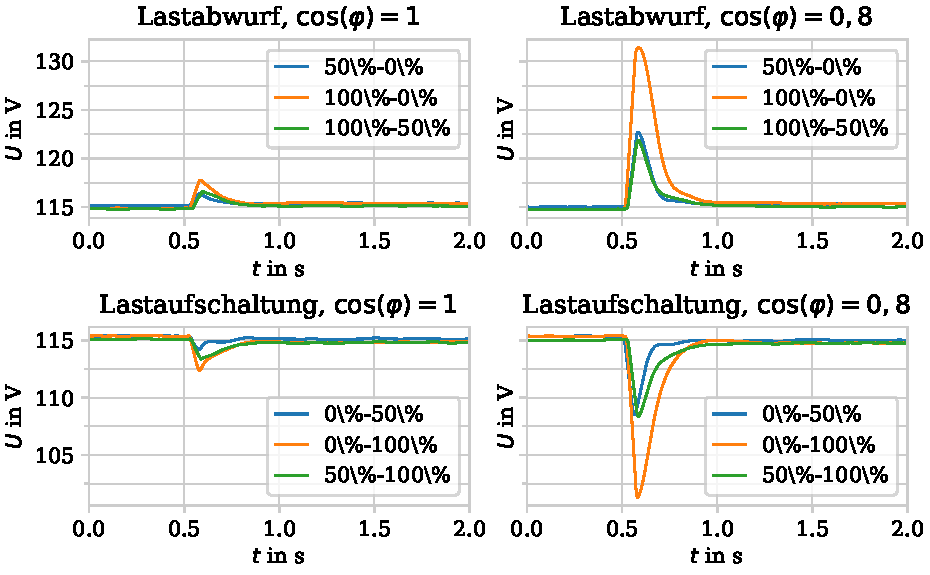
\includegraphics{Bilder/DynamischeMessung.pdf}
	\caption{Zeitverläufe der dynamischen Messung}
	\label{fig:ZeitverlaufDynamischOhneRegleraenderung}
\end{figure}

\section{Parameter und Zeitverläufe der Dynamischen Messung mit Reglerveränderung}
\label{sec:ReglerparameterDynamischeMessung}

\begin{longtable}[]{ll}
    \caption{Veränderter D-Anteil (Standardwert: $\mathrm{UgenCtrlD_G}=27648$)}
    \label{tab:Parameter-D-Messung}
    \tabularnewline
    \toprule
    Versuch     & $\mathrm{UgenCtrlD_G}$ \\
    \midrule
    \endfirsthead
    \toprule
    Versuch     & $\mathrm{UgenCtrlD_G}$ \\
    \midrule
    \endhead    
    9.1.1.1.1/2 & 26112        \\
    9.1.1.2.1/2 & 26880        \\
    9.1.1.3.1/2 & 28160        \\
    9.1.1.4.2 & 29184        \\
    9.1.4.6.1/2 & 256          \\
    9.1.4.6.3/5 & 5376         \\
    9.1.4.6.4/6 & 13824        \\
    9.1.4.6.7/8 & 20736        \\
    \bottomrule
\end{longtable}

\begin{longtable}[]{ll}
    \caption{Veränderter I-Anteil (Standardwert: $\mathrm{UgenCtrlI_G}=304$))}
    \label{tab:Parameter-I-Messung}
    \tabularnewline
    \toprule
    Versuch     & $\mathrm{UgenCtrlI_G}$ \\
    \midrule
    \endhead
        9.1.2.1.1/2 & 0            \\
        9.1.2.2.1/2 & 152          \\
        9.1.2.3.1/2 & 456          \\
        9.1.2.4.1/2 & 608          \\
        9.1.2.6.1/2 & 912          \\
    \bottomrule
\end{longtable}

\begin{longtable}[]{lll}
    \caption{Veränderter konstanter P-Anteil, eingestellt mit Begrenzung des PP-Glieds,\\Standardwerte: $\mathrm{UgenCtrlPP_G}=2048$, $\mathrm{UgenCtrlPP_{UL}}=8192$, $\mathrm{UgenCtrlPP_{LL}}=6144$)}
    \label{tab:Parameter-P-Messung}
        \tabularnewline
    \toprule
    Versuch     & $\mathrm{UgenCtrlPP_{LL}}$ & $\mathrm{UgenCtrlPP_{UL}}$ \\
    \midrule
    \endfirsthead
    \caption{Veränderter konstanter P-Anteil, eingestellt mit Begrenzung des PP-Glieds,\\Standardwerte: $\mathrm{UgenCtrlPP_G}=2048$, $\mathrm{UgenCtrlPP_{UL}}=8192$, $\mathrm{UgenCtrlPP_{LL}}=6144$)}
    \tabularnewline
    \toprule
    Versuch     & $\mathrm{UgenCtrlPP_{LL}}$ & $\mathrm{UgenCtrlPP_{UL}}$ \\
    \midrule
    \endhead
        9.1.3.1.1/2 & 3072         & 3072  \\
        9.1.3.2.1/2 & 4608         & 4608  \\
        9.1.3.3.1/2 & 8192         & 8192  \\
        9.1.3.4.1/2 & 12288        & 12288 \\
    \bottomrule
\end{longtable}

\begin{longtable}[]{lll}
    \caption{PI-Regler mit veränderten konstanten Verstärkungen, eingestellt mit Begrenzung des PP-Glieds,\\Standardwerte: siehe \cref{tab:Parameter-P-Messung},\\D-Glied ausgeschaltet: $\mathrm{UgenCtrlD_G=0}$}
    \label{tab:Parameter-PI-Messung}
    \tabularnewline
    \toprule
    Versuch     & $\mathrm{UgenCtrlPP_{LL}}$ & $\mathrm{UgenCtrlPP_{UL}}$ \\
    \midrule
    \endhead
        9.1.3.1.1/2 & 3072         & 3072  \\
        9.1.3.2.1/2 & 4608         & 4608  \\
        9.1.3.3.1/2 & 6144         & 6144  \\
        9.1.3.4.1/2 & 12288        & 12288 \\
    \bottomrule
\end{longtable}

\begin{landscape}
\begin{figure}
    \centering
    \oldincludegraphics[]{Bilder/MessungReglerSweep.pdf}
    \caption{Zeitverläufe der dynamischen Messung mit Reglerveränderung}
    \label{fig:MessungReglerSweep}
\end{figure}
\end{landscape}

\section{Zeitverläufe der Spannungen aus den Parameterstudien}
\begin{figure}[!ht]
    \centering
    \begin{subfigure}{\linewidth}
        \centering
        \oldincludegraphics[width=\textheight-2.5in, angle=90]{Bilder/ParameterSweep.pdf}
        \subcaption{Hauptinduktivitäten, Statorstreuinduktivitäten}
        \label{fig:InduktivitatenSweepA}
    \end{subfigure}
    \caption{Zeitverläufe der simulierten Spannungen aus der Parameterstudie der Induktivitäten. Die Legende rechts gibt die Farbzuordnung zu dem ausgewerteten Punkt. Aufgetragen sind 10er-Schritte aus der Parameterstudie}
\end{figure}

\begin{figure}[ht]\ContinuedFloat
    \begin{subfigure}{\textwidth}
        \centering
        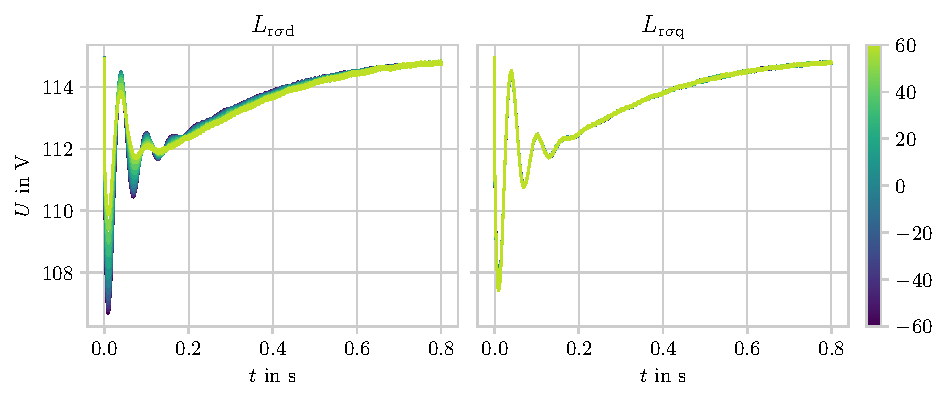
\includegraphics{Bilder/ParameterSweep_RotorStreuinduk.pdf}
        \subcaption{Rotorstreuinduktivitäten des Synchrongenerators. Aufgetragen sind 10er-Schritte aus der Parameterstudie.}
        \label{fig:InduktivitatenSweepB}
    \end{subfigure}
    \begin{subfigure}{\textwidth}
        \centering
        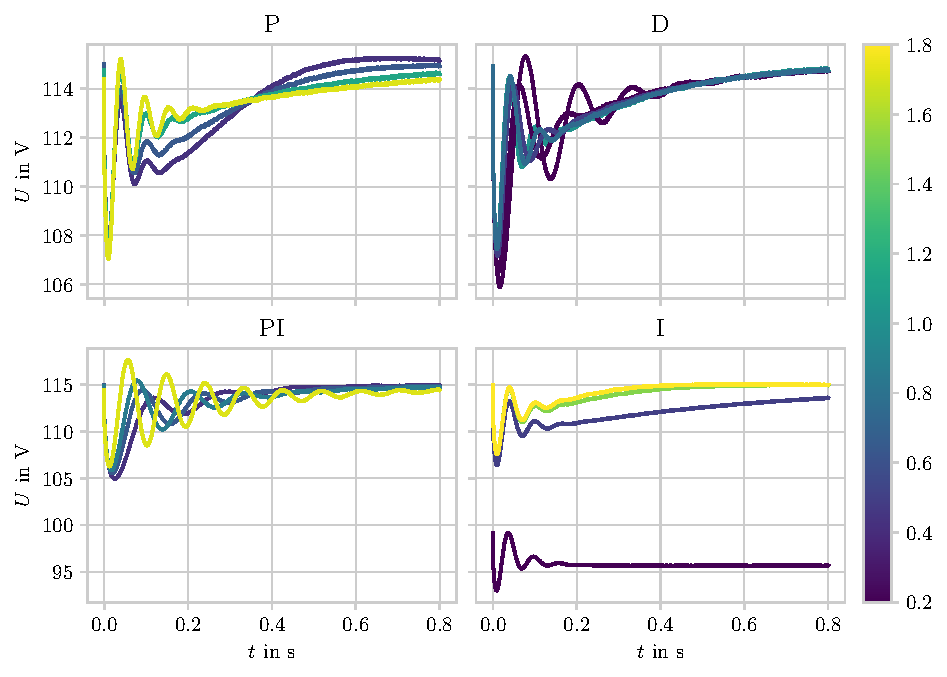
\includegraphics{Bilder/simulation_reglerSweepSpannungen.pdf}
        \subcaption{Reglerparameter. Die Legende rechts gibt den jeweiligen Variationsfaktor einer Kurve}
    \label{fig:SpannungenReglerSweep}
    \end{subfigure}
    \caption{Zeitverläufe der simulierten Spannungen aus der Parameterstudie.}
    \label{fig:ZeitverlauefeSpannungenParametersweep}
\end{figure}
